\documentclass[border=10pt]{standalone}
\usepackage{pgf,tikz,pgfplots}
\usetikzlibrary{quotes, angles}
\usetikzlibrary{positioning}
\usetikzlibrary{arrows.meta}
\usetikzlibrary{calc, shapes, automata, fit}
\tikzset{%
	% Specifications for style of nodes:
	base/.style = {rectangle, rounded corners, draw=black,
		%		minimum width=4cm, minimum height=1cm,
		inner sep=15pt,
		text centered, font=\sffamily}, 
	activityStarts/.style = {base, fill=blue!30},
	startstop/.style = {base, fill=red!30},
	activityRuns/.style = {base, fill=red!30},
	process/.style = {base, minimum width=2.5cm, fill=orange!15,
		font=\ttfamily},
	context/.style = {base, inner sep=5pt, align=justify, fill=blue!30}
}
\begin{document}
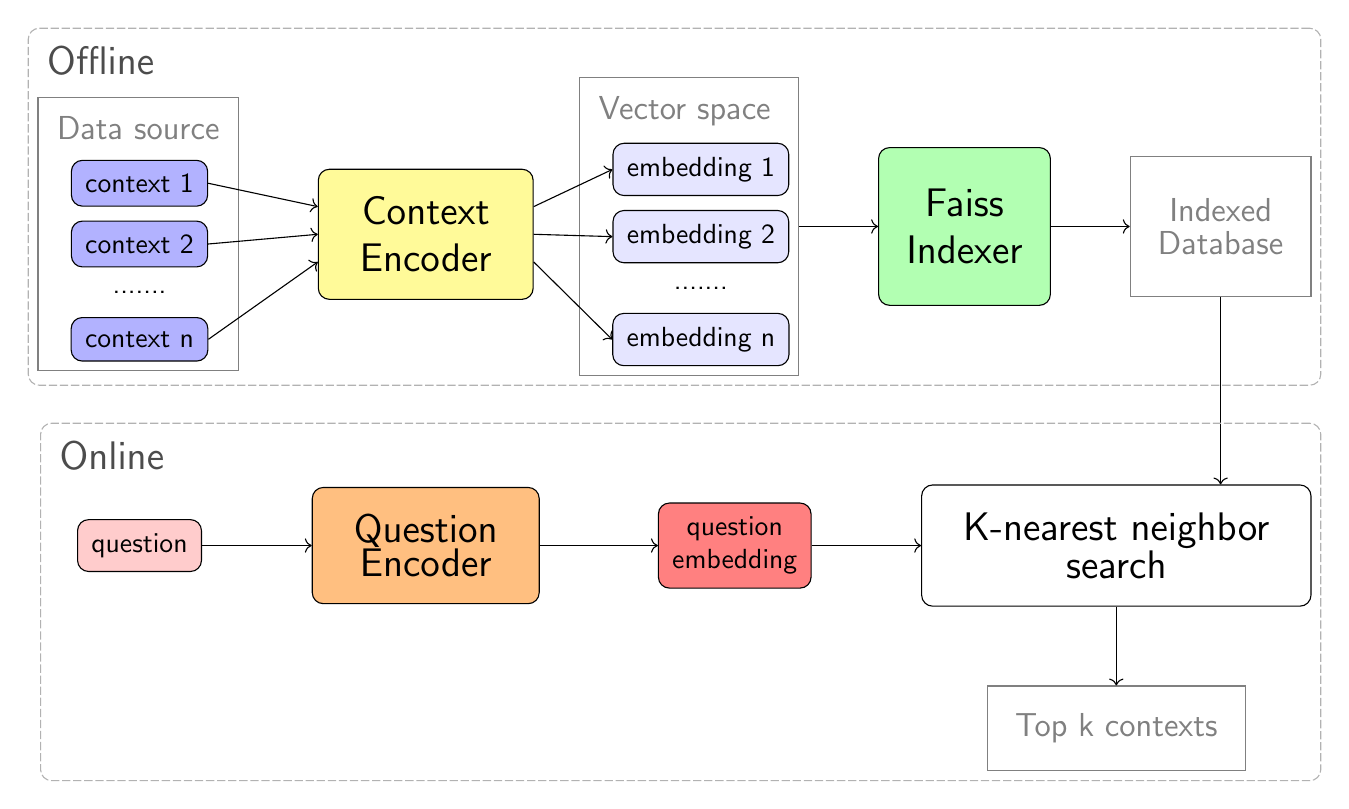
\begin{tikzpicture}[every node/.style={font=\sffamily}, align=center]
	\node (ctxs1) [context] {context 1};
	\node (ctxs2) [context, below=5pt of ctxs1] {context 2};
	\node (dots) [below=5pt of ctxs2] {.......};
	\node (ctxsn) [context, below=5pt of dots] {context n};
	\path let
		\p1 = (ctxs1.north),
		\p2 = (ctxs1.west)
	in
		coordinate (northCtxs) at (\x2, \y1);
	\node (dataSource) [anchor=west, shift={(-0.3cm, 0.4cm)}, font=\fontsize{12pt}{\baselineskip}\selectfont\color{black!50}\sffamily] at (northCtxs) {Data source};
	\node [draw=black!50, fit={(dataSource) (ctxs1) (ctxs2) (dots) (ctxsn)}] (contextBlock) {};
	\node (contextEncoder) [align=center, right=1cm of contextBlock, inner xsep=15pt, inner ysep=10pt, fill=yellow!40, draw=black, rounded corners] {\fontsize{14pt}{\baselineskip}\selectfont Context\\[5pt]\fontsize{14pt}{\baselineskip}\selectfont Encoder};
	\draw[->] (ctxs1.east) -- ([yshift=10pt]contextEncoder.west);
	\draw[->] (ctxs2.east) -- (contextEncoder.west);
	\draw[->] (ctxsn.east) -- ([yshift=-10pt]contextEncoder.west);
	\path let
		\p1 = (contextEncoder.east),
		\p2 = (ctxs1)
	in
		coordinate (embAnchor) at (\x1 + 1cm, \y2);
	\node (ctxEmb1) [anchor=west, fill=blue!10, rounded corners, draw=black, inner sep=5pt, yshift=5pt] at (embAnchor) {embedding 1};
	\node (ctxEmb2) [fill=blue!10, rounded corners, draw=black, below=5pt of ctxEmb1, inner sep=5pt] {embedding 2};
	\node (embDots) [below=5pt of ctxEmb2] {.......};
	\node (ctxEmbn) [anchor=west, fill=blue!10, rounded corners, draw=black, below=5pt of embDots, inner sep=5pt] {embedding n};
	\path let
		\p1 = (ctxEmb1.north),
		\p2 = (ctxEmb1.west)
	in
		coordinate (ctxEmbAnchor) at (\x2, \y1);
	\node (vecSpace) [anchor=west, shift={(-0.3cm, 0.4cm)}, font=\fontsize{12pt}{\baselineskip}\selectfont\color{black!50}\sffamily] at (ctxEmbAnchor) {Vector space};
	\node (vecSpaceBlock) [fit={(vecSpace) (ctxEmbn)}, draw=black!50] {};
	\draw[->] ([yshift=10pt]contextEncoder.east) -- (ctxEmb1.west);
	\draw[->] (contextEncoder.east) -- (ctxEmb2.west);
	\draw[->] ([yshift=-10pt]contextEncoder.east) -- (ctxEmbn.west);
	\node (faissIndexer) [right=1cm of vecSpaceBlock, rounded corners, fill=green!30, inner xsep=10pt, inner ysep=15pt, draw=black] {\fontsize{14pt}{\baselineskip}\selectfont Faiss\\[5pt] \fontsize{14pt}{\baselineskip}\selectfont Indexer};
	\draw[->] (vecSpaceBlock.east) -- (faissIndexer.west);
	\node [right=1cm of faissIndexer, draw=black!50, font=\fontsize{12pt}{\baselineskip}\selectfont\color{black!50}\sffamily, inner xsep=10pt, inner ysep=15pt] (indexedDB) {Indexed\\ Database};
	\draw[->] (faissIndexer.east) -- (indexedDB.west);
	\node (offlineLabel) [above=2.2cm of contextBlock.west, anchor=west, font=\fontsize{14pt}{\baselineskip}\selectfont\color{black!70}\sffamily] {Offline};
	\node (offline) [rounded corners, dash pattern=on 3pt off 1pt,fit={(offlineLabel) (contextBlock) (vecSpaceBlock) (indexedDB)}, draw=black!30] {};
	\node (question) [rounded corners, fill=red!20, draw=black, below=2cm of ctxsn, inner sep=5pt] {question};
	\path let
		\p1 = (question),
		\p2 = (contextEncoder)
	in
		coordinate (questionEncoder) at (\x2, \y1);
	\node (questionEncoder) [rounded corners, fill=orange!50, inner xsep=15pt, inner ysep=10pt, font=\fontsize{14pt}{\baselineskip}\selectfont\sffamily, draw=black] at (questionEncoder) {Question\\ Encoder};
	\draw[->] (question) -- (questionEncoder);
	\node (questionEmb) [rounded corners, fill=red!50, draw=black, inner sep=5pt, right=1.5cm of questionEncoder] {question \\embedding};
	\draw[->] (questionEncoder) -- (questionEmb);
	\path let
		\p1 = (indexedDB.east),
		\p2 = (questionEmb.east)
	in
		coordinate (knnAnchor) at (\x1, \y2);
	\node (knn) [anchor=east, inner xsep=15pt, inner ysep=10pt, rounded corners, font=\fontsize{14pt}{\baselineskip}\selectfont\sffamily, draw=black] at (knnAnchor) {K-nearest neighbor\\search};
	\path let
		\p1 = (knn.north),
		\p2 = (indexedDB.south)
	in
		coordinate (knnAnchorNorth) at (\x2, \y1);
	\draw[->] (indexedDB.south) -- (knnAnchorNorth);
	\draw[->] (questionEmb) -- (knn);
	\node (topK) [below=1cm of knn, draw=black!50, font=\fontsize{12pt}{\baselineskip}\selectfont\color{black!50}\sffamily,inner sep=10pt] {Top k contexts};
	\draw[->] (knn) -- (topK);
	\node (onlineLabel) [above=0.5cm of question, xshift=-10pt, font=\fontsize{14pt}{\baselineskip}\selectfont\color{black!70}\sffamily] {Online};
	\node (online) [rounded corners, dash pattern=on 3pt off 1pt, draw=black!30, fit={(onlineLabel) (questionEncoder) (questionEmb) (knn) (topK)}] {};
\end{tikzpicture}
\end{document}